\documentclass[11pt, a4paper]{article}

\usepackage{graphicx}
\usepackage[a4paper,top=3cm,bottom=2cm,left=2cm,right=2cm,marginparwidth=1.75cm]{geometry}
\usepackage[english]{babel}
\usepackage[utf8x]{inputenc}
\usepackage{subfig}
\usepackage{float}
\usepackage{amsmath}
\usepackage{amssymb}
\usepackage{mhchem}
\usepackage{hyperref}
\usepackage{tikz}
\usepackage{cancel}

\graphicspath{ {./images} }
\newcommand*{\qed}{\hfill\ensuremath{\quad\square}}%
\newcommand*{\rad}{\ensuremath{\,\text{rad}}}
\newcommand*{\R}{\ensuremath{\mathbb{R}}}
\newcommand*{\C}{\ensuremath{\mathbb{C}}}
\renewcommand*{\Re}{\operatorname{Re}}
\renewcommand*{\Im}{\operatorname{Im}}
\renewcommand*{\epsilon}{\varepsilon}
\renewcommand*{\phi}{\varphi}

\makeatletter
\renewcommand*\env@matrix[1][*\c@MaxMatrixCols c]{%
  \hskip -\arraycolsep
  \let\@ifnextchar\new@ifnextchar
  \array{#1}}
\makeatother

\newtheorem{theorem}{Theorem}

%------------------------------------------------
%Templates for images and figures
% \begin{figure}[h]
%   \centering
%   \subfloat[caption 1]{{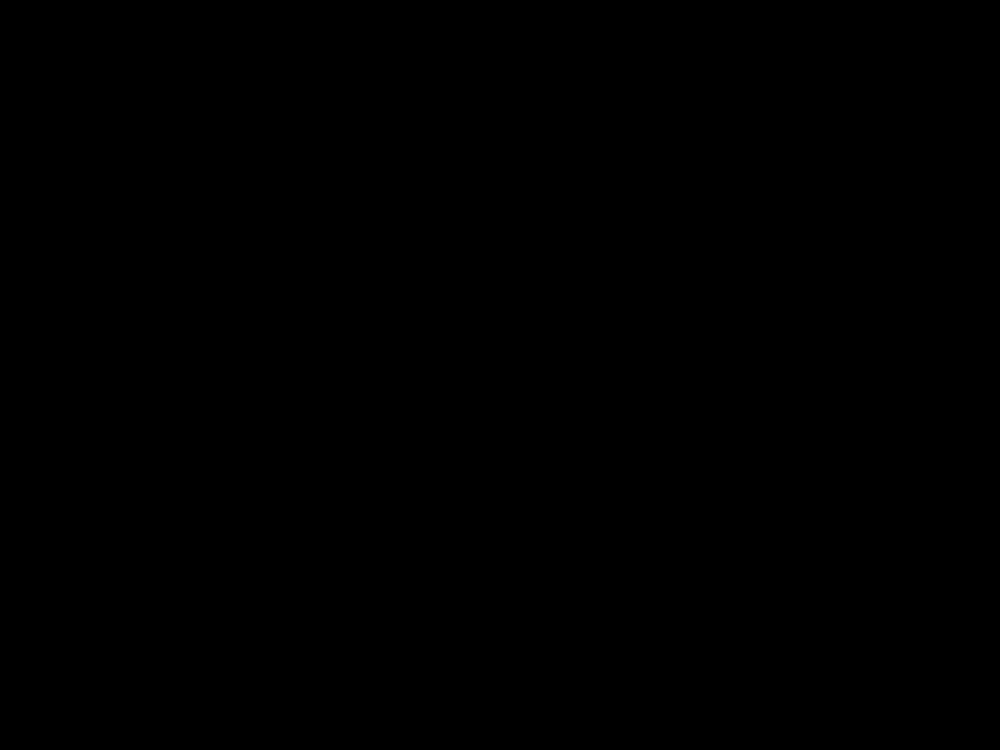
\includegraphics[width=30mm]{images/placeholder.png}}}%
%   \qquad
%   \subfloat[caption 2]{{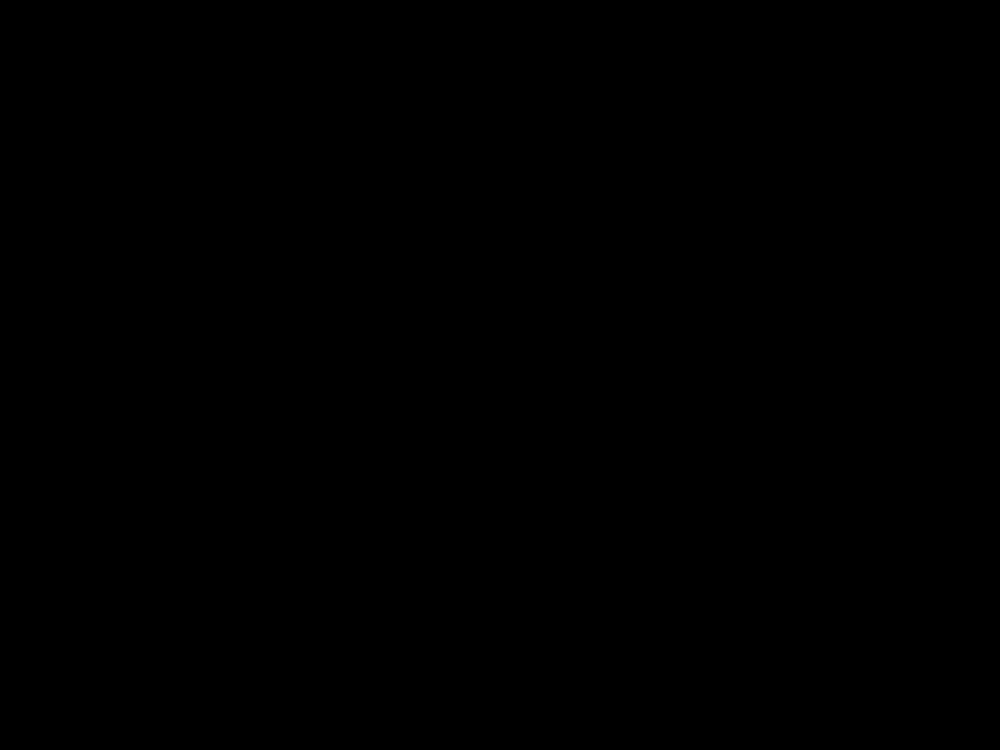
\includegraphics[width=30mm]{images/placeholder.png}}}%
%   \caption{Description}
% \end{figure}

% \begin{figure}[h]
%   \centerline{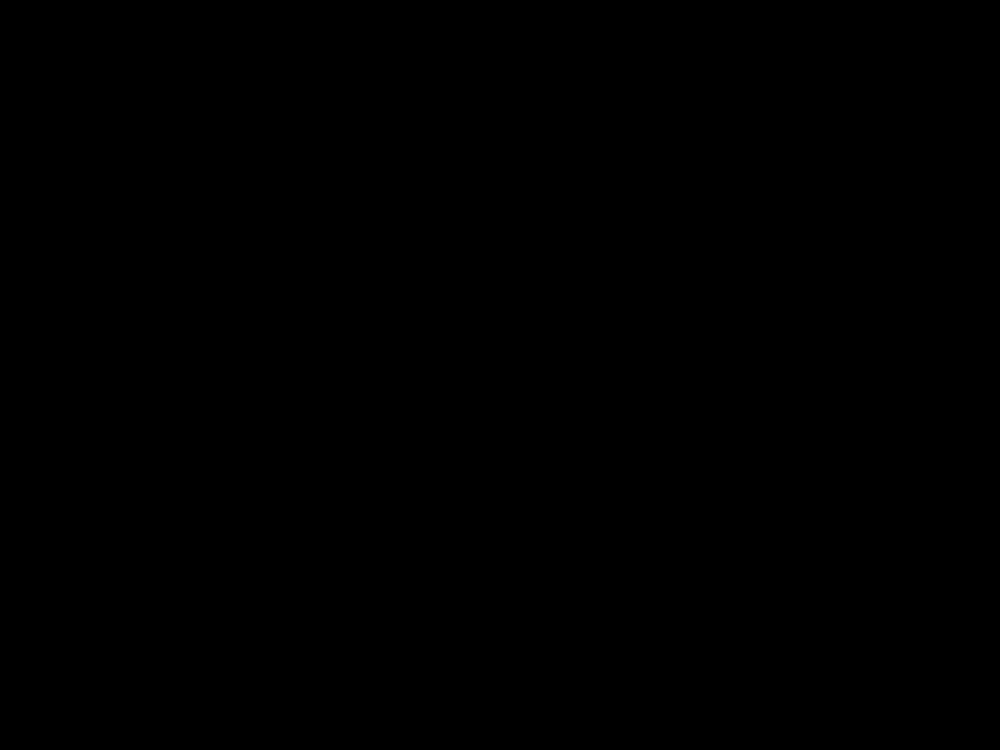
\includegraphics[width=50mm]{images/placeholder.png}}
%   \caption{Description}
% \end{figure}

%Template for a simple table 
%\begin{table}[h]
%   \caption{Description} %title of the table
%   \centering % centering table
%   \begin{tabular}{l rr} % creating three columns
%     \hline\hline %inserting double-line
%     & & \\ [0.5ex] % Insert half line vertical spacing
%     \hline % inserts single-line
%     & & \\ 
%     & & \\
%     & & \\
%     & & \\
%   \hline % inserts single-line
%   \end{tabular}
%   \label{tab:hresult}
% \end{table}
%-----------------------------------------------

\begin{document}
\setcounter{equation}{0}
\setcounter{section}{11}

\section{Thermofluids Lecture 12: Vapor Power Cycles (04/06/2020)}

\subsection{Defining vapor power cycles and the rankine cycle}
A vapor power cycle refers to a type of power cycle where the working fluid is alternitly vaporized and condensed. The working fluid for these type of cycles is usually water/steam for it's high enthalpy of vaporization and low cost. Examples of power generation through the usage of steam power are nuclear plants, natural gas plants, coal plants and geothermal plants. In general steam power plants consist of some type of pump, a boiler, a turbine and a condensor.
\begin{figure}[h]
  \centerline{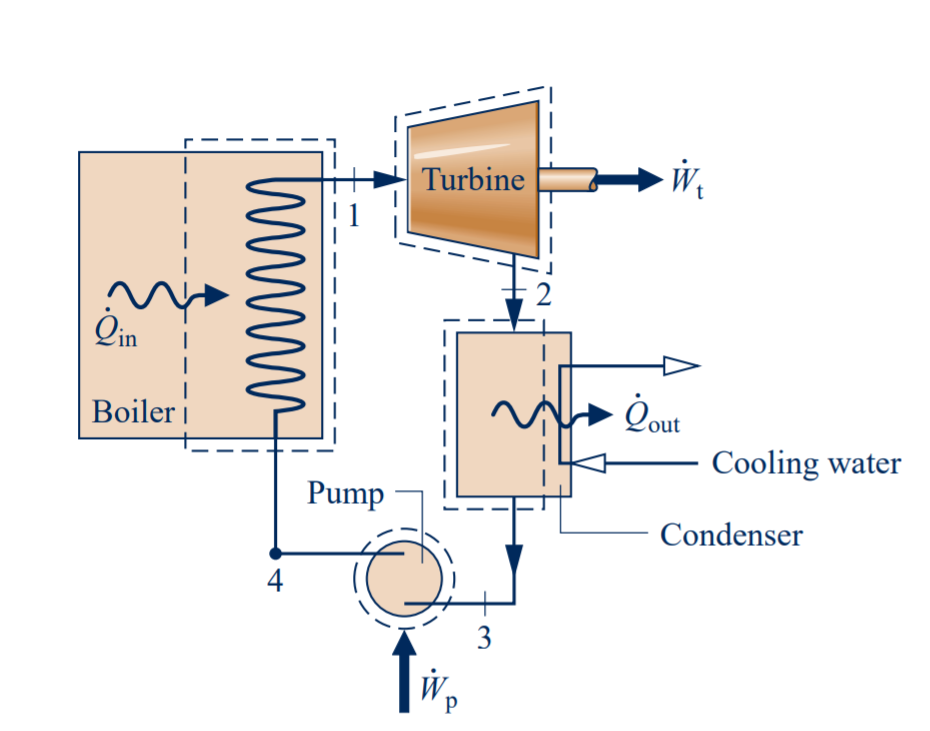
\includegraphics[width=80mm]{images/Schematic.png}}
  \caption{A typical setup for a vapor power cycle with a pump, condensor, turbine and boiler.}
\end{figure}
The Rankine-cycle is an idealized vapor power cycle for vapor power generation. We use a different idealized cycle because the Carnot-cycle does make for a realistic model when considering vapor power cycles. The Rankine power cycle has 4 steps:
\begin{itemize}
  \item $1 \to 2$: Isentropic compression in a pump
  \item $2 \to 3$: Constant-pressure heat addition in a boiler 
  \item $3 \to 4$: Isentropic expansion in a turbine
  \item $4 \to 1$: Constant-pressure heat rejection in a condensor
\end{itemize}
A simple $T-s$-diagram for an ideal Rankine cycle is shown in figure \ref{fig:RankineCycle}.
\begin{figure}[h]
  \centerline{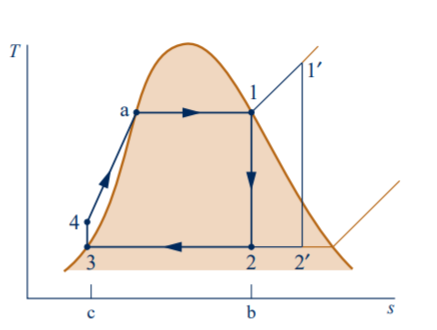
\includegraphics[width=80mm]{images/RankineCycle.png}}
  \caption{The $T-s$-diagram for an idealized Rankine cycle}
  \label{fig:RankineCycle}
\end{figure}


\subsection{Mass and energy rate balance applied to the devices of a Rankine cycle}
The following equations can be derrived by assuming steady-flow and applying the first law for an open system.
\begin{table}[h]
  \caption{The equations for devices in a Rankine vapor cycle} %title of the table
  \centering % centering table
  \begin{tabular}{l|l} % creating three columns
    \hline\hline %inserting double-line
    Device & Equation\\ [0.5ex] % Insert half line vertical spacing
    \hline \hline
    Turbine & $\frac{\dot{W}_t}{\dot{m}} = h_1 - h_2$ \\ 
    Condensor &  $\frac{\dot{Q}_{out}}{\dot{m}} = h_2 - h_3$\\
    Pump &  $\frac{\dot{W}_p}{\dot{m}} = h_4 - h_3$, $\left( \frac{\dot{W}_p}{\dot{m}} \right)_s \approx v_3(p_4 - p_3)$\\
    Boiler & $\frac{\dot{Q}_{in}}{\dot{m}} = h_1 - h_4$ \\
  \hline % inserts single-line
  \end{tabular}
  \label{tab:hresult}
\end{table}
Subscript $s$ is used to denote an isentropic process. An isentropic is a process which is both adiabatic and internally reversable.
\end{document}